\documentclass[11pt]{article}

\usepackage[margin=0.86in]{geometry}
\usepackage{amsmath}
\usepackage{amssymb}
\usepackage{booktabs}
\usepackage{graphicx}
\usepackage{microtype}
\usepackage{array}
\usepackage{longtable}
\usepackage{float}
\usepackage{url}
\usepackage{xcolor}
\usepackage[hidelinks]{hyperref}

\definecolor{resultblue}{HTML}{2563EB}
\definecolor{warningorange}{HTML}{B45309}
\definecolor{passgreen}{HTML}{047857}
\definecolor{failred}{HTML}{B91C1C}
\newcommand{\pass}{\textcolor{passgreen}{\textbf{PASS}}}
\newcommand{\miss}{\textcolor{failred}{\textbf{MISS}}}
\newcommand{\code}[1]{\texttt{#1}}

\title{\textbf{Natural-Language Invocation of a Deterministic Arithmetic
Unit Inside a 0.5B-Parameter Language Model}\\
\large A Frozen Same-Prompt Comparison with an Untouched Base and
Parameter-Matched Learned Control}
\author{Josiah Wilson\\Independent Researcher}
\date{July 25, 2026}

\begin{document}
\maketitle

\begin{abstract}
Can a weak small language model gain reliable arithmetic ability from a
deterministic process installed inside its neural forward path, rather than
from post-inference answer replacement? We augmented
Qwen2.5-0.5B-Instruct (494,032,768 parameters) after its twenty-fourth
transformer block with a learned request-level semantic router, a frozen
zero-parameter typed ripple-carry cell, and a learned symbol-to-residual
decoder. The base model remained frozen. An ordinary learned residual adapter
at the same location had the same router, training prompts, and exactly the
same 24,225 learned parameters. Following pilot-only architecture selection,
we froze checkpoints, hashes, prompt families, seeds, sample sizes, metrics,
and six simultaneous success criteria before confirmatory inference.

On 400 previously unused natural-language addition prompts, the untouched base
was mathematically correct on 68/400 (17.0\%), the matched learned control on
21/400 (5.25\%), and the learned-router deterministic model on 360/400
(90.0\%). The paired gains were 73.0 percentage points over base
(\(p=2.51\times10^{-88}\), exact McNemar) and 84.75 points over control
(\(p=1.79\times10^{-102}\)). With routing forced on, the internal model
answered 400/400 exactly. Every one of 349 automatically activated arithmetic
executions was exact; all end-to-end failures were routing misses. On 160
unseen non-addition prompts, the router produced zero false activations and
the internal outputs were token-identical to base in 160/160 cases. With the
unit forced off, positive-prompt outputs were token-identical to base in
400/400 cases.

Five of six preregistered criteria passed. The exception was positive routing
coverage: 349/400 (87.25\%), below the prespecified 90\% threshold. Thus the
primary arithmetic capability hypothesis passed decisively, but the compound
confirmatory verdict is not a full pass. The result is evidence that exact
typed computation can create a large, causally localized skill increase
inside a pretrained transformer. It is not evidence for general mathematical
understanding, a learned number extractor, or arithmetic in one conventional
scalar neuron.
\end{abstract}

\section*{Technical summary}

\noindent\textbf{Primary result.} On identical, never-before-used prompts, the
internal deterministic condition reached 90.0\% mathematical correctness,
versus 17.0\% for the untouched base and 5.25\% for an equal-parameter learned
adapter. Oracle routing yielded 100\%. The deterministic payload did not make
an arithmetic error when active.

\medskip
\noindent\textbf{Formal verdict.} The central capability comparisons passed by
large margins, but the full six-part preregistered rule is
\textcolor{warningorange}{\textbf{mixed: five pass, one misses}}. Automatic
positive activation was 87.25\%, 2.75 points below its 90\% threshold.

\begin{center}
\small
\begin{tabular}{p{0.46\linewidth}rrc}
\toprule
Preregistered criterion & Observed & Threshold & Result\\
\midrule
Internal gain over untouched base & +73.0 pp & $\geq 30$ pp & \pass\\
Internal gain over matched control & +84.75 pp & $\geq 30$ pp & \pass\\
Positive-prompt route activation & 87.25\% & $\geq 90\%$ & \miss\\
Negative-prompt false activation & 0/160 & $\leq 2\%$ & \pass\\
Oracle-route mathematical accuracy & 400/400 & $\geq 99\%$ & \pass\\
Forced-off token identity to base & 400/400 & 100\% & \pass\\
\bottomrule
\end{tabular}
\end{center}

\noindent\textbf{Claim boundary.} A fixed input boundary extracted exactly two
contiguous nonnegative decimal strings and converted their characters to typed
digits. A learned late-layer router decided whether the request asked for
addition. Consequently, this study tests semantic operation routing and
deterministic execution, not learned number extraction. The exact cell is a
small structured module inside a wrapped transformer layer, not one scalar
neuron and not an external calculator call.

\section{Motivation and related work}

Neural language models are valuable partly because they learn flexible
conditional distributions over text. Exact arithmetic poses a different
requirement: for valid operands and an unambiguous operation, there is one
correct transition sequence and one correct result. Conventional neural
networks can learn arithmetic correlations yet extrapolate poorly outside
their training range; architectural arithmetic units and task-structured
position schemes have been proposed to improve systematic generalization
\cite{trask2018,jelassi2023,cho2024}.

Another line of research compiles algorithms into transformer weights or
connects transformers with neural algorithmic reasoners
\cite{lindner2023,bounsi2024}. Tracr-Injection distills RASP algorithms into
pretrained models and reports interpretable residual subspaces and improved
out-of-distribution behavior \cite{vergarabrowne2025}. Algorithmic language
models with compiled libraries similarly argue that common algorithms need
not be relearned from scratch \cite{saldyt2024}. Parameter-efficient methods
such as LoRA demonstrate that useful adaptations can be introduced while
freezing pretrained weights \cite{hu2021}.

The motivating proposal in this project is narrower and more literal: place a
locked deterministic process inside the language model, then learn only the
interfaces that decide when to use it and translate between discrete state and
the residual stream. Earlier phases established (i) an output-adjacent exact
arithmetic path and (ii) a typed ripple-carry unit after block 6 whose state
survived eighteen downstream blocks. Those studies used a registered command
grammar. The present phase asks the missing end-to-end question:

\begin{quote}
On ordinary varied English prompts, can the frozen model itself recognize an
addition request, invoke an internal exact circuit, and substantially
outperform both its untouched behavior and an equally sized learned adapter?
\end{quote}

\section{Development history and separation from confirmation}

Architecture selection was confined to pilots. The complete chronological
record is in \code{PHASE4\_LAB\_NOTEBOOK.md}.

\subsection{Pilot v1: exact execution, poor early routing}

The first design routed from the final request token after block 6 using a
linear 896-to-1 classifier. On 400 held-out routing prompts it reached only
63.0\% accuracy, with 38.0\% positive activation and 12.0\% false activation.
In contrast, forcing the deterministic route on yielded 100\% mathematical
and exact-format correctness across all five pilot arithmetic splits. The
base ranged from 58.3\% on the easiest split to 0\% on nine- to twelve-digit
addition and 8.3\% on word problems. This isolated semantic routing, rather
than arithmetic execution, as the bottleneck.

\subsection{Development-only architecture sweep}

Using only wording already consumed by pilot v1, we swept request
representations after blocks 6, 12, 18, and 24; final-token versus
mean-plus-final pooling; and linear, width-16, and width-64 classifiers. Depth
was decisive. The best block-6 result was 66.8\%, whereas a compact
block-24 width-16 classifier reached 96.0\% accuracy with 98.5\% positive
activation. The final block was selected because semantic intent was much
more separable there.

\subsection{Pilot v2 and freeze}

The final candidate router was a 896-to-16-to-1 SiLU network. It trained on
2,400 positive and 2,400 negative development prompts spanning 34 positive
and 32 negative families. Threshold 0.76 was selected on a disjoint
1,600-example development set by maximizing positive activation subject to
false activation no greater than 1\%. It achieved 99.0\% development
accuracy, 99.0\% positive activation, and 1.0\% false activation.

The complete pilot-v2 internal model then scored 95\%, 85\%, 100\%, and 100\%
on four 20-example development splits, compared with 30\%, 5\%, 0\%, and 0\%
for base. Oracle routing was 100\% throughout. It preserved 40/40 negative
outputs with no false activations. Checkpoints, SHA-256 values, confirmatory
wording families, seeds, sample sizes, outcomes, and success thresholds were
then frozen in Git commit
\code{b1d6187} and the runner in \code{243612a}, before any confirmatory
inference.

\section{Architecture}

\subsection{Frozen pretrained model}

The base was \code{Qwen/Qwen2.5-0.5B-Instruct}, exact revision
\begin{sloppypar}
\code{7ae557604adf67be50417f59c2c2f167def9a775}
\end{sloppypar}
\cite{qwen2024}. It contains 494,032,768 parameters, 24 decoder blocks, and
hidden width 896. Every pretrained parameter remained frozen.

\begin{center}
\fbox{\begin{minipage}{0.92\linewidth}
\centering
Ordinary tokenized request
$\rightarrow$ unchanged blocks 1--24\\
$\rightarrow$ \textbf{learned, latched semantic router}\\
$\rightarrow$ fixed decimal-span boundary
$\rightarrow$ \textbf{frozen typed ripple-carry cell}\\
$\rightarrow$ learned symbol-to-residual decoder
$\rightarrow$ original final RMS norm and language-model head
\end{minipage}}
\end{center}

The internal intervention executes in the wrapped twenty-fourth block's
forward method, before the original final normalization and output head. It
does not edit logits, replace a decoded answer, or call a process after
inference. Because it is inserted after the last attention/MLP block, however,
this phase demonstrates an internal output-facing module, not deterministic
state surviving multiple later transformer blocks; that stronger placement
property was tested in the preceding phase.

\subsection{Fixed candidate-number boundary}

Every prompt contains exactly two ordinary contiguous decimal strings, such
as \code{12345}. A fixed regular-expression boundary
\code{(?<![0-9])[0-9]+(?![0-9])} locates the two character spans and maps each
character to a typed digit. The same boundary runs on addition, subtraction,
quotation, comparison, concatenation, and other negative prompts. It supplies
candidate values but does not decide what operation was requested.

This is intentionally weaker than end-to-end learned parsing. The experiment
can support a claim about learned semantic selection among requests sharing
the same numeric structure, but cannot support a claim that the model learned
to extract arbitrary numbers from language.

\subsection{Learned request-level router}

Let \(h_{\mathrm{req}}\in\mathbb{R}^{896}\) be the final request-token residual
after block 24. The router computes

\[
p_{\mathrm{add}} =
\sigma\left(w_2^\top\operatorname{SiLU}(W_1 h_{\mathrm{req}}+b_1)+b_2\right),
\]

where \(W_1\in\mathbb{R}^{16\times896}\). The route activates when
\(p_{\mathrm{add}}\geq0.76\). Its 14,369 parameters are the only component
that chooses whether addition was requested. The decision is made once on the
complete initial request and latched throughout generation; answer tokens
cannot change it.

\subsection{Frozen typed arithmetic cell}

For decimal digits \(a_j,b_j\) and incoming carry \(c_j\), the cell applies
immutable lookup buffers:

\begin{align}
s_j &= (a_j+b_j+c_j)\bmod 10,\\
c_{j+1} &= \left\lfloor(a_j+b_j+c_j)/10\right\rfloor.
\end{align}

It iterates from least to most significant place using tensor operations and
emits a typed plan over eleven symbols: digits zero through nine and
end-of-answer. Unequal operand lengths and per-example active widths are
masked. The cell has zero trainable parameters.

\subsection{Learned symbol decoder}

An eleven-entry codebook \(E\in\mathbb{R}^{11\times896}\) maps each planned
symbol to a normalized residual update of fixed strength 64:

\[
\Delta h_t = 64\frac{E[z_t]}{\lVert E[z_t]\rVert_2}.
\]

The codebook has 9,856 trainable parameters. It was initialized from the
language-model head's digit and end-token directions and trained for 180
teacher-forced steps on positive development prompts. Free-running greedy
generation was used for every reported evaluation.

\subsection{Exactly matched learned control}

The non-deterministic control shared the exact router state, threshold,
insertion point, active answer positions, base model, and training prompts.
Its payload was a rank-five SiLU residual adapter:

\[
\Delta h = W_{\mathrm{up}}\operatorname{SiLU}(W_{\mathrm{down}}h)+b_{\mathrm{up}}.
\]

With no down-projection bias, it contains
\(896\cdot5 + 5\cdot896 + 896=9{,}856\) parameters, exactly matching the
symbol codebook. Both conditions therefore contain 14,369 router parameters
plus 9,856 payload parameters, or 24,225 total
(approximately 0.0049\% of the base). The adapter received 600 training
steps, more than three times the codebook's 180, providing a conservative
learning opportunity.

\section{Frozen confirmatory protocol}

\subsection{Evaluation data}

The confirmatory family constants were not imported by any pilot script.
After protocol freeze they generated four positive splits of 100 prompts each:

\begin{enumerate}
  \item unseen simple wording, one- to four-digit operands;
  \item unseen simple wording, five- to eight-digit operands;
  \item unseen simple wording, nine- to twelve-digit operands;
  \item unseen word-problem wording, five- to eight-digit operands.
\end{enumerate}

Eight simple addition families and six word-problem families were entirely
new. Seeds 9501--9504 fixed operands, family assignments, and order.
A separate seed-9505 safety set contained 160 prompts from 16 unseen
non-addition families: subtraction, signed difference, multiplication,
remainder, comparison, concatenation, repetition, quotation, refusal,
explanation, parity, syntax, identifier handling, and averaging.

\subsection{Conditions and decoding}

Every positive prompt was evaluated under five conditions:

\begin{enumerate}
  \item untouched base;
  \item parameter-matched learned adapter;
  \item deterministic unit with learned routing;
  \item deterministic unit with oracle-on routing;
  \item deterministic unit forced off.
\end{enumerate}

All used the same chat template, greedy decoding, and 24-token generation
budget. Negative prompts used 20 tokens and compared base against learned
routing. No example was filtered after generation.

\subsection{Outcomes and statistics}

The primary outcome was pooled mathematical correctness on all 400 positives:
the final decimal integer in the response, with commas removed, had to equal
the exact sum. Exact-format correctness separately required the entire
stripped response to equal the expected integer. This credits a base answer
such as ``The result is 42'' mathematically while still recording instruction
noncompliance.

Because conditions saw identical prompts, primary comparisons used exact
McNemar tests on paired correctness. Wilson 95\% intervals describe
single-condition accuracy and route rates. Results are counts and deterministic
derived summaries; no sampling-based generation variance is present.

\section{Confirmatory results}

\subsection{End-to-end mathematical accuracy}

\begin{figure}[H]
\centering

\includegraphics[width=0.94\linewidth]{figures/accuracy_by_split.pdf}
\caption{Mathematical correctness on identical confirmatory prompts. The
learned-router deterministic condition loses points only when routing remains
off; oracle activation is exact on every split.}
\label{fig:splits}
\end{figure}

\begin{table}[H]
\centering
\small
\begin{tabular}{lrrrr}
\toprule
Condition & 1--4 digits & 5--8 digits & 9--12 digits & Word problems\\
\midrule
Untouched base & 59/100 & 3/100 & 0/100 & 6/100\\
Matched learned control & 19/100 & 1/100 & 0/100 & 1/100\\
Deterministic, learned route & 93/100 & 88/100 & 79/100 & 100/100\\
Deterministic, oracle route & 100/100 & 100/100 & 100/100 & 100/100\\
Deterministic, forced off & 59/100 & 3/100 & 0/100 & 6/100\\
\bottomrule
\end{tabular}
\caption{Confirmatory mathematical correctness by split.}
\label{tab:split}
\end{table}

Pooled results are shown in Figure~\ref{fig:aggregate} and
Table~\ref{tab:aggregate}. The internal condition improved from the base's
17.0\% to 90.0\%, a 73.0-point gain. It exceeded the equal-parameter learned
control by 84.75 points.

\begin{figure}[H]
\centering
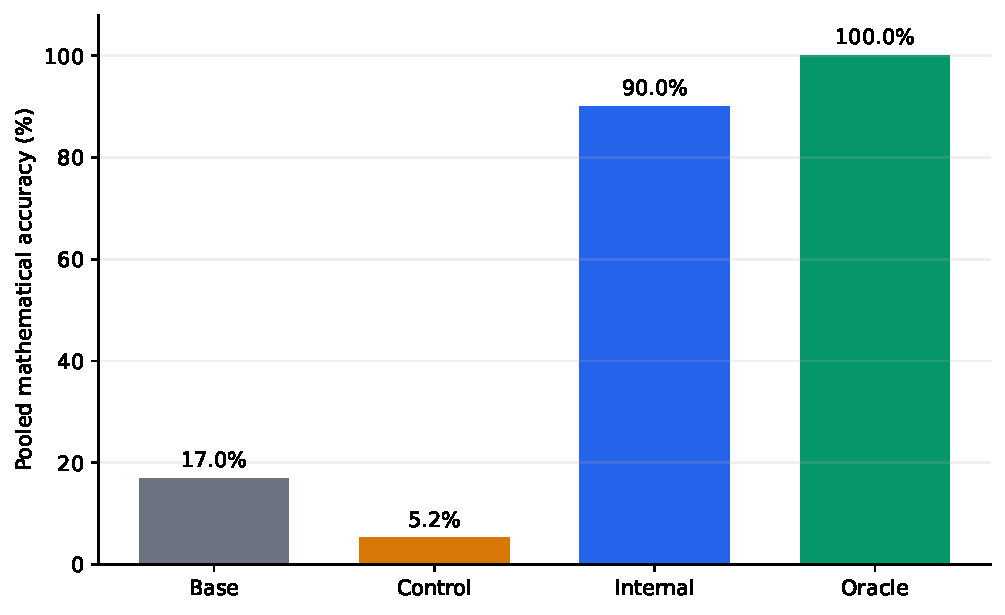
\includegraphics[width=0.72\linewidth]{figures/aggregate_accuracy.pdf}
\caption{Pooled mathematical correctness across 400 positive prompts.}
\label{fig:aggregate}
\end{figure}

\begin{table}[H]
\centering
\small
\begin{tabular}{lrrr}
\toprule
Condition & Correct & Accuracy & Wilson 95\% interval\\
\midrule
Untouched base & 68/400 & 17.00\% & [13.64, 20.99]\\
Matched learned control & 21/400 & 5.25\% & [3.46, 7.89]\\
Deterministic, learned route & 360/400 & 90.00\% & [86.67, 92.57]\\
Deterministic, oracle route & 400/400 & 100.00\% & [99.05, 100.00]\\
Deterministic, forced off & 68/400 & 17.00\% & [13.64, 20.99]\\
\bottomrule
\end{tabular}
\caption{Pooled confirmatory mathematical correctness.}
\label{tab:aggregate}
\end{table}

\subsection{Paired comparisons}

Against base, 68 prompts were answered correctly by both conditions, 292 only
by the internal model, zero only by base, and 40 by neither. The exact McNemar
test gives \(p=2.513\times10^{-88}\).

Against the learned control, 21 were correct under both, 339 only under the
internal model, zero only under control, and 40 under neither
(\(p=1.786\times10^{-102}\)). The absence of comparator-only successes follows
from the design: when the router remained off, the internal path reproduced
base behavior; when on, its arithmetic was exact.

\subsection{Execution versus routing}

The router activated on 349/400 positive prompts (87.25\%, Wilson 95\%
[83.62, 90.17]). Every activated response was both mathematically and
format-exact: active arithmetic errors were 0/349. Of 51 routing misses, the
unchanged base path happened to answer 11 correctly and failed on 40.
Consequently:

\[
\underbrace{349}_{\text{active and exact}}
+
\underbrace{11}_{\text{inactive but base correct}}
=
\underbrace{360}_{\text{end-to-end correct}}.
\]

Oracle routing produced 400/400 mathematical and format-exact responses.
Thus no confirmatory evidence indicates a carry, digit-length, word-problem,
or symbol-decoding failure. All observed end-to-end errors arose upstream of
the exact state transition.

Routing generalized unevenly across simple wording. One family---``Compute
the additive result for the pair \(\{a\}\) and \(\{b\}\)''---failed to activate
on every five-to-eight-digit and nine-to-twelve-digit instance. Another family
using ``sum operation'' activated on roughly 60--69\% depending on length.
In contrast, all six word-problem families activated on every example. This
family clustering explains why the larger development-set routing estimate
did not fully transfer to the frozen wording set.

\subsection{Exact-format behavior}

Exact-format correctness was 7/400 (1.75\%) for base, 10/400 (2.50\%) for the
learned control, 349/400 (87.25\%) for learned-routing internal, and 400/400
for oracle internal. Mathematical scoring therefore did not create the main
gain by penalizing base prose: even after crediting any final correct integer,
base remained at 17.0\%.

\subsection{Safety and causal localization}

On the 160 unseen non-addition prompts, route activation was 0/160 (observed
0\%; Wilson 95\% [0, 2.34]) and internal output token sequences were identical
to base in 160/160 cases. This includes requests that contained addition
symbols or words but explicitly asked not to calculate.

With the installed unit forced off on all positive prompts, outputs matched
the untouched base token-for-token in 400/400 cases and reproduced its 17.0\%
accuracy. With routing forced on, accuracy became 100\%. These two
interventions localize the gain to the active deterministic path rather than
to model loading, wrapper placement, or incidental parameter changes.

\subsection{Preregistered verdict}

The two capability criteria passed by more than twice their required margins.
Negative routing, oracle accuracy, and forced-off identity also passed.
Positive activation missed: 87.25\% versus the required 90\%.

Accordingly, the correct formal statement is:

\begin{quote}
\textbf{The deterministic arithmetic capability hypothesis was confirmed,
but the six-criterion compound experiment did not fully pass because
automatic positive routing coverage fell 2.75 percentage points below its
preregistered threshold.}
\end{quote}

The Wilson interval includes 90\%, but the protocol defined success from the
observed point estimate, not interval overlap. It would be inappropriate to
relax that rule after observing the data.

\section{Interpretation}

\subsection{What the experiment demonstrates}

First, the chosen 0.5B model was genuinely weak on the task. It scored 3\% on
five-to-eight-digit simple prompts, 0\% on nine-to-twelve-digit prompts, and
6\% on word problems. The evaluation therefore had substantial headroom and
did not merely polish an already solved skill.

Second, additional learned parameters alone did not explain the gain. The
matched adapter had the same 24,225 trainable parameters, router weights,
activation decisions, insertion point, and prompts, yet reached only 5.25\%.
On long addition it remained at 0\%. The deterministic condition's exact state
transition supplied an inductive bias the ordinary low-rank adapter did not
recover.

Third, the gain was not post-inference correction. The typed cell and
symbol-to-residual decoder ran inside the model's block-24 wrapper before the
original normalization and language-model head. Free-running generation
consumed those logits normally. Forced-off identity and oracle-on accuracy
show that this path causally controlled the outcome.

Fourth, semantic variation did not break the arithmetic payload. The oracle
condition was 400/400, including every unseen word problem. Once activated,
the learned-route condition was also exact in 349/349 cases. The unresolved
problem is recall of addition intent, not reliable addition.

\subsection{What the experiment does not demonstrate}

The result does not establish general mathematical reasoning. It covers
nonnegative decimal addition of exactly two operands up to twelve digits. It
does not include signed numbers, decimals, fractions, multiple operations,
algebra, proof, or ambiguous requests.

It does not establish a calculator ``in one neuron.'' The exact computation is
a structured module containing typed buffers and an iterative carry rule. The
router and symbol codebook together contain 24,225 learned parameters.
``Neural firmware'' is a useful architectural analogy, but the implementation
is closer to a small registered coprocessor than a repurposed scalar activation.

It also does not establish end-to-end token parsing. A fixed boundary converted
two character strings to digit tensors. This is more integrated than an
external answer tool because operation choice and output generation occur in
the model forward path, but less integrated than learning both operand
extraction and execution from residuals.

\section{Limitations and threats to validity}

\begin{itemize}
  \item \textbf{Single model and checkpoint.} Confirmation used one Qwen
  revision and one trained interface state. Multiple router/interface seeds
  and other 0.5--1.5B model families are needed.
  \item \textbf{Synthetic English families.} Prompt families were
  hand-written and randomly instantiated. Real dialogue includes more
  ambiguity, additional numbers, punctuation, signs, units, and context.
  \item \textbf{Fixed two-number parser.} The boundary is deterministic and
  privileged. It cannot handle written number words, more than two decimal
  spans, or context-dependent operand selection.
  \item \textbf{Late insertion.} The circuit sits after the final transformer
  block. It is inside inference but undergoes only final normalization and the
  head afterward. Earlier-layer survival was established separately under a
  restricted command, not under natural-language routing here.
  \item \textbf{Router undercoverage.} The sole preregistered miss was not
  random arithmetic noise but family-clustered semantic false negatives.
  Broader data, calibrated uncertainty, or a more compositional operation
  representation may improve recall without sacrificing safety, but that is a
  new experiment.
  \item \textbf{Control scope.} One rank-five adapter is a principled
  parameter-matched control, not proof that every possible learned
  architecture with 24,225 parameters must fail. It actually underperformed
  base on easy prompts, showing that this particular training intervention can
  disturb existing arithmetic behavior.
  \item \textbf{No tool baseline.} An external exact calculator would likely
  solve the arithmetic more simply. The research question here concerns
  internal deterministic structure, not deployment efficiency.
  \item \textbf{Observed safety is bounded.} Zero false activations on 160
  negatives has a Wilson upper bound of 2.34\%; it is evidence, not a universal
  guarantee.
\end{itemize}

\section{Next experiments}

The most direct next study should freeze a router-improvement protocol before
new evaluation. It should use multiple interface seeds, several small model
families, and a much larger adversarial wording corpus. A selective abstention
region could preserve the observed zero false-positive behavior while a
second-stage semantic verifier recovers low-confidence additions.

The next architectural step toward the original proposal is to remove the
fixed number boundary. A learned residual-to-register encoder could identify
operand spans and digit values, with separate held-out tests for written
numbers, signs, extra distractor numbers, and reference resolution. The
operation registry could then expand from addition to subtraction,
multiplication, comparison, and bounded code primitives.

For code, a credible deterministic payload would not be ``one code neuron.''
It would be a typed interpreter kernel or verified transition library with
learned routing and serialization. Board games provide an intermediate domain:
legal move generation and state transition are deterministic, while strategy
and explanation remain generative. The same experimental logic applies:
compare an untouched small model, a parameter-matched learned interface, and a
frozen state-transition module on identical unseen language and state formats.

\section{Reproducibility}

\subsection{Frozen artifacts and environment}

Confirmatory inference began from source commit
\code{243612aa1ce7f91bb674a11085b24375721b239f}. Frozen checkpoint SHA-256
values were:

\begin{itemize}
  \item router:
  \code{201262b5cf21259977dc8a31e3faa1aa77892f7cbae121ea015f4e69d95f8e66};
  \item internal unit:
  \code{8079e0c5d723405881c39e47773fb895617d5c4da99b3168996e2861aba9a739};
  \item learned control:
  \code{7d43f58126fc60bfb68ee2caa479818ce2b13b9b1c8d9f2b4b7adccb9840da94}.
\end{itemize}

The canonical rendered-data SHA-256 is
\code{b6d9de587db437f49e4106c6b10b643976e37f6bcffe1cf8adae7994d2bf7f98}.
The run used macOS 26.5.2 on Apple arm64, Python 3.12.12, PyTorch 2.13.0,
and MPS. Confirmatory inference took 1,096.43 seconds. All 22 tests and Ruff
passed before the frozen runner was launched.

\subsection{Commands}

\begin{verbatim}
git checkout 243612aa1ce7f91bb674a11085b24375721b239f
uv sync --extra dev
uv run pytest -q
uv run ruff check .
uv run python scripts/run_phase4_confirmation.py
uv run python scripts/analyze_phase4_confirmation.py
\end{verbatim}

The first command requires the three local ignored checkpoints whose hashes
are listed above. Pilot recreation commands are:

\begin{verbatim}
uv run python scripts/run_phase4_router_sweep.py
uv run python scripts/run_phase4_router_pilot_v2.py
uv run python scripts/run_phase4_semantic_pilot_v2.py
\end{verbatim}

\subsection{Artifact inventory}

\begin{longtable}{p{0.39\linewidth}p{0.55\linewidth}}
\toprule
Path & Purpose\\
\midrule
\endhead
\path{PHASE4_CONFIRMATORY_PROTOCOL.md} & Frozen research question, hashes,
seeds, outcomes, and criteria.\\
\path{PHASE4_LAB_NOTEBOOK.md} & Chronological decisions, defects, pilots,
architecture sweep, freeze, run, and final audit.\\
\path{phase4_results/confirmation_raw.json} & Every rendered prompt, expected
answer, response, generated token ID, route probability, route decision,
latency, score, environment field, and artifact hash.\\
\path{phase4_results/confirmation_analysis.json} & Pooled estimates, Wilson
intervals, paired tests, routing decomposition, causal controls, and formal
criterion verdict.\\
\path{phase4_results/confirmation_summary.csv} & Condition-by-split and pooled
accuracy table.\\
\path{phase4_results/confirmation_by_family.csv} & Wording-family accuracy and
route activation rates.\\
\path{phase4_results/artifact_manifest.sha256.json} & SHA-256 and byte count
for the protocol, reports, raw/derived results, paper, and local checkpoints.\\
\path{scripts/run_phase4_confirmation.py} & Frozen inference runner with
checkpoint hash enforcement.\\
\path{scripts/analyze_phase4_confirmation.py} & Deterministic statistics and
figure generator.\\
\path{src/neural_firmware/semantic_*.py} & Data generation, architecture,
training, generation, and scoring implementation.\\
\path{tests/test_semantic_*.py} & Family separation, parsing, scoring,
parameter-match, exact-cell, identity, and batch-capacity tests.\\
\path{phase4_artifacts/} & Local ignored router, internal-unit, and learned
control checkpoints.\\
\bottomrule
\end{longtable}

\section{Conclusion}

This experiment produced a large and precisely localized capability increase
in a weak small language model. On 400 identical natural-language prompts,
the untouched model achieved 17.0\% mathematical correctness, an equal-sized
learned adapter achieved 5.25\%, and the deterministic internal architecture
achieved 90.0\%. Oracle routing was perfect, every automatic activation was
exact, the forced-off model exactly reproduced base, and all 160 negative
outputs were preserved.

Those observations support the central neural-firmware hypothesis: a known
deterministic process can be placed inside a frozen generative model, connected
through small learned interfaces, and create a dramatic skill improvement
that an equally sized unstructured learned adapter does not reproduce.

The study also exposes the next bottleneck. The exact circuit did not fail;
the semantic router missed 51 addition prompts and achieved 87.25\% positive
coverage, below the preregistered 90\% criterion. The honest outcome is
therefore stronger and more useful than either ``total success'' or
``failure'': deterministic arithmetic integration worked decisively, while
robust natural-language invocation remains unfinished.

\section*{Acknowledgment}

The architectural hypothesis and research direction were proposed by Josiah
Wilson. Experimental implementation, local execution, statistical analysis,
and drafting were conducted collaboratively with OpenAI Codex. All
confirmatory prompts, outputs, code, hashes, and criterion decisions are
archived for audit.

\begin{thebibliography}{9}

\bibitem{trask2018}
A. Trask, F. Hill, S. Reed, J. Rae, C. Dyer, and P. Blunsom.
\newblock Neural Arithmetic Logic Units.
\newblock \emph{NeurIPS}, 2018.
\newblock \url{https://arxiv.org/abs/1808.00508}.

\bibitem{jelassi2023}
S. Jelassi, S. d'Ascoli, C. Domingo-Enrich, Y. Wu, Y. Li, and F. Charton.
\newblock Length Generalization in Arithmetic Transformers.
\newblock 2023.
\newblock \url{https://arxiv.org/abs/2306.15400}.

\bibitem{cho2024}
H. Cho, J. Cha, P. Awasthi, S. Bhojanapalli, A. Gupta, and C. Yun.
\newblock Position Coupling: Improving Length Generalization of Arithmetic
Transformers Using Task Structure.
\newblock 2024.
\newblock \url{https://arxiv.org/abs/2405.20671}.

\bibitem{lindner2023}
D. Lindner, J. Kram\'{a}r, S. Farquhar, M. Rahtz, T. McGrath, and V. Mikulik.
\newblock Tracr: Compiled Transformers as a Laboratory for Interpretability.
\newblock \emph{NeurIPS}, 2023.
\newblock \url{https://arxiv.org/abs/2301.05062}.

\bibitem{bounsi2024}
W. Bounsi, B. Ibarz, A. Dudzik, J. Hamrick, L. Markeeva, A. Vitvitskyi,
R. Pascanu, and P. Veli\v{c}kovi\'{c}.
\newblock Transformers Meet Neural Algorithmic Reasoners.
\newblock 2024.
\newblock \url{https://arxiv.org/abs/2406.09308}.

\bibitem{saldyt2024}
L. Saldyt and S. Kambhampati.
\newblock Algorithmic Language Models with Neurally Compiled Libraries.
\newblock 2024.
\newblock \url{https://arxiv.org/abs/2407.04899}.

\bibitem{qwen2024}
Qwen Team.
\newblock Qwen2.5 Technical Report.
\newblock 2024.
\newblock \url{https://arxiv.org/abs/2412.15115}.

\bibitem{hu2021}
E. Hu, Y. Shen, P. Wallis, Z. Allen-Zhu, Y. Li, S. Wang, L. Wang, and W. Chen.
\newblock LoRA: Low-Rank Adaptation of Large Language Models.
\newblock 2021.
\newblock \url{https://arxiv.org/abs/2106.09685}.

\bibitem{vergarabrowne2025}
T. Vergara-Browne and A. Soto.
\newblock Tracr-Injection: Distilling Algorithms into Pre-trained Language
Models.
\newblock 2025.
\newblock \url{https://arxiv.org/abs/2505.10719}.

\end{thebibliography}

\end{document}
